\chapter{Results and Discussions}\label{cap:results}


\section{Experimental Testing Methodology}\label{section:testingMethodology}

There were performed some tests on the the reservoirs from the \gls{SCMB} and the system integrated worked well. Although some difficulties were presented, principally due the format of the thread pitch, the 3D device model was able to fit in the openings of the plastic drum barrels, and the measurements could be taken from the detergent surface level.

In order to characterize the developed measurement system, as demonstrated in Figure~\ref{fig:flowchartUltrasonicReadings}, some experimental tests were performed with the objective of verifying the system's accuracy. For this purpose, the device was submitted to take 50 measurements from an object surface, as can been in Figure~\ref{fig:measurementTesting}, and four tests were performed with eight different distances, within a range of 5 cm to 400 cm. For each test, it was varied the filter size, which is responsible for the ultrasonic sensor to take successively measurements, in a short period of time, and to return the mean of these values.

\begin{figure}[h!]
    \centering
    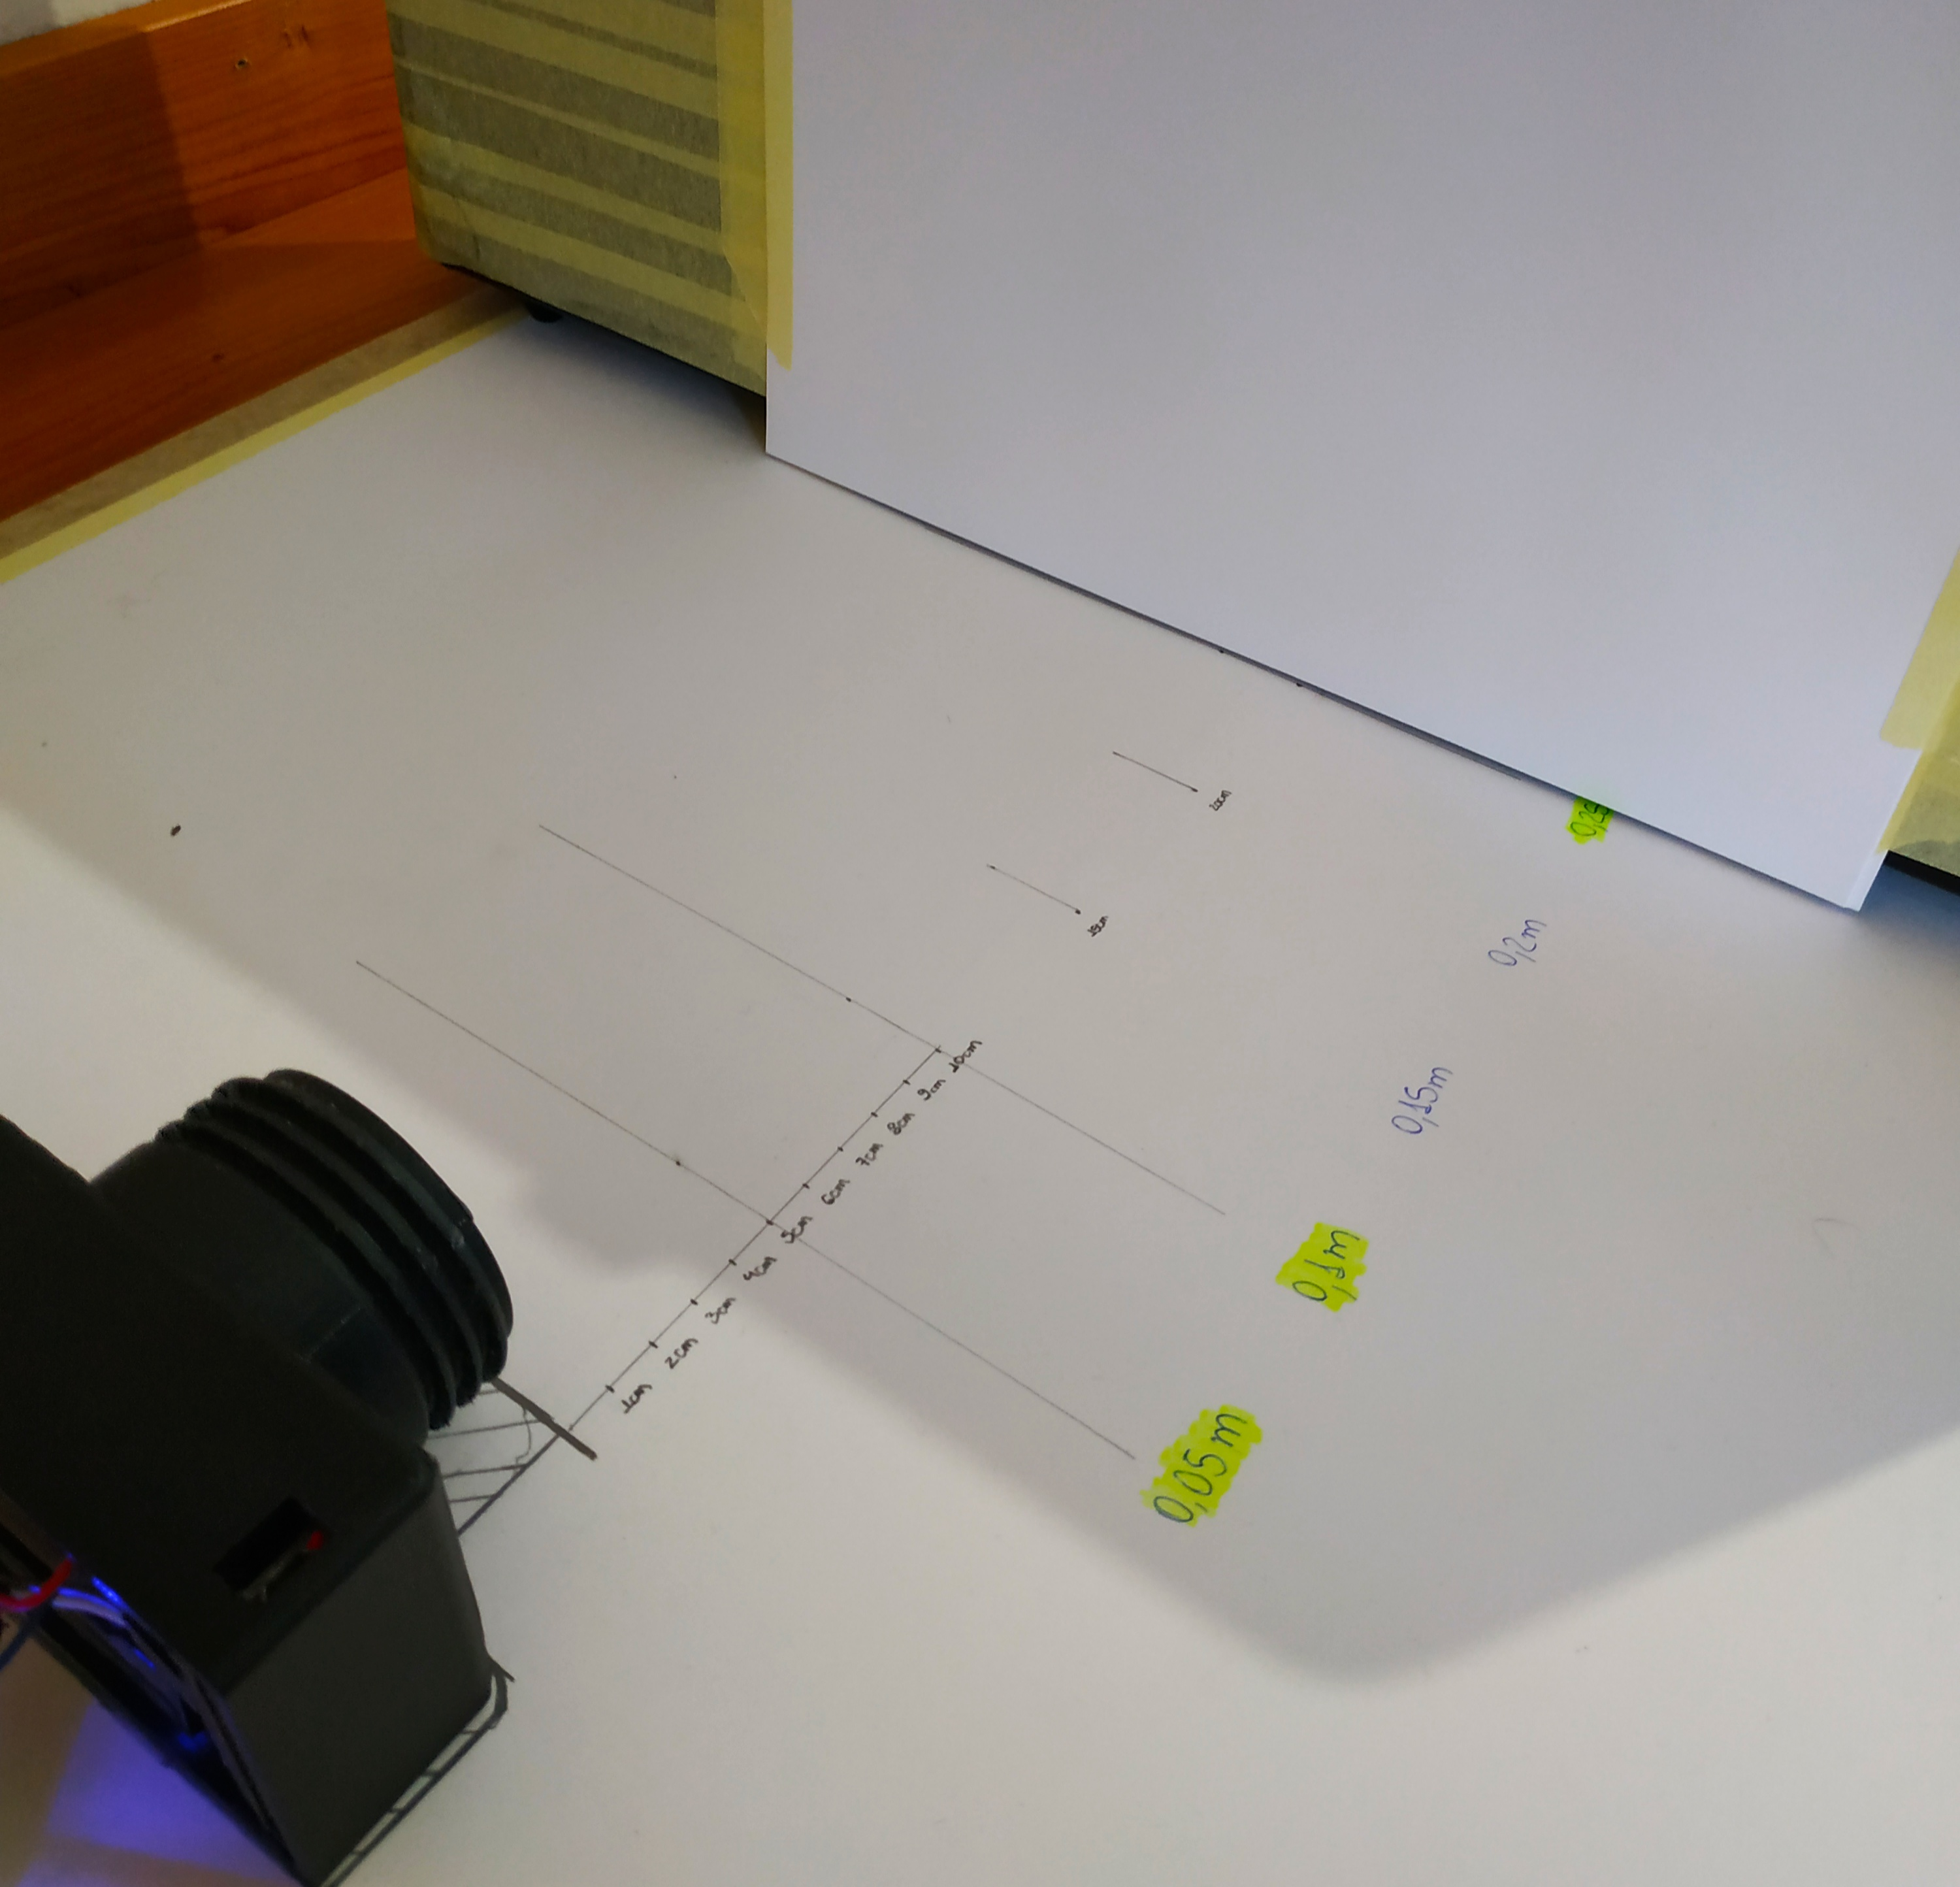
\includegraphics[scale=0.075]{images/Results/testing_methodology/3Dtesting.jpg}
    \caption{Elaborate scenario for the test measurement systems.}
    \label{fig:measurementTesting}
\end{figure}

Table~\ref{table:testSummary} shows the distances and values for each test realized. It is important to point out that these tests were performed in a controlled environment where the temperature was a known factor. 

\begin{table}[h!]
    \centering
    \begin{tabular}{@{}ccc@{}}
        \toprule
        \textbf{Tests} & \textbf{Distances (cm)} & \textbf{Filter Size} \\ \midrule
        \rowcolor[HTML]{EFEFEF} 
        A & 5/10/25/50/100/200/300/400 & 1 \\
        B & 5/10/25/50/100/200/300/400 & 5 \\
        \rowcolor[HTML]{EFEFEF} 
        C & 5/10/25/50/100/200/300/400 & 20 \\ 
        D & 5/10/25/50/100/200/300/400 & 50 \\ \bottomrule
    \end{tabular}
    \caption{Summary of the experimental tests with different distances being measured.}
    \label{table:testSummary}
\end{table}


\subsection{Analysis of the Experimental Results}

The tests performed will be presented in this subsection. Due to the large quantity of information, only some of them will be provided, however, sufficient for the analysis of the results. The rest of the tests can be found in Appendix \ref{appendice1:first}.

In Figure~\ref{fig:50cmText}, it is presented the measurement results with the object placed in a distance of 50~cm from the sensor. The first thing that can be noticed is the high value of the average systematic error presented. Although it is an inherent characteristic from any measurement process, its high value is mostly influenced due to the offset adopted for the system, in which it is considered the zero point as the beginning of the device thread, and not from the ultrasonic sensor itself.

\begin{figure}[h!]
    \centering
    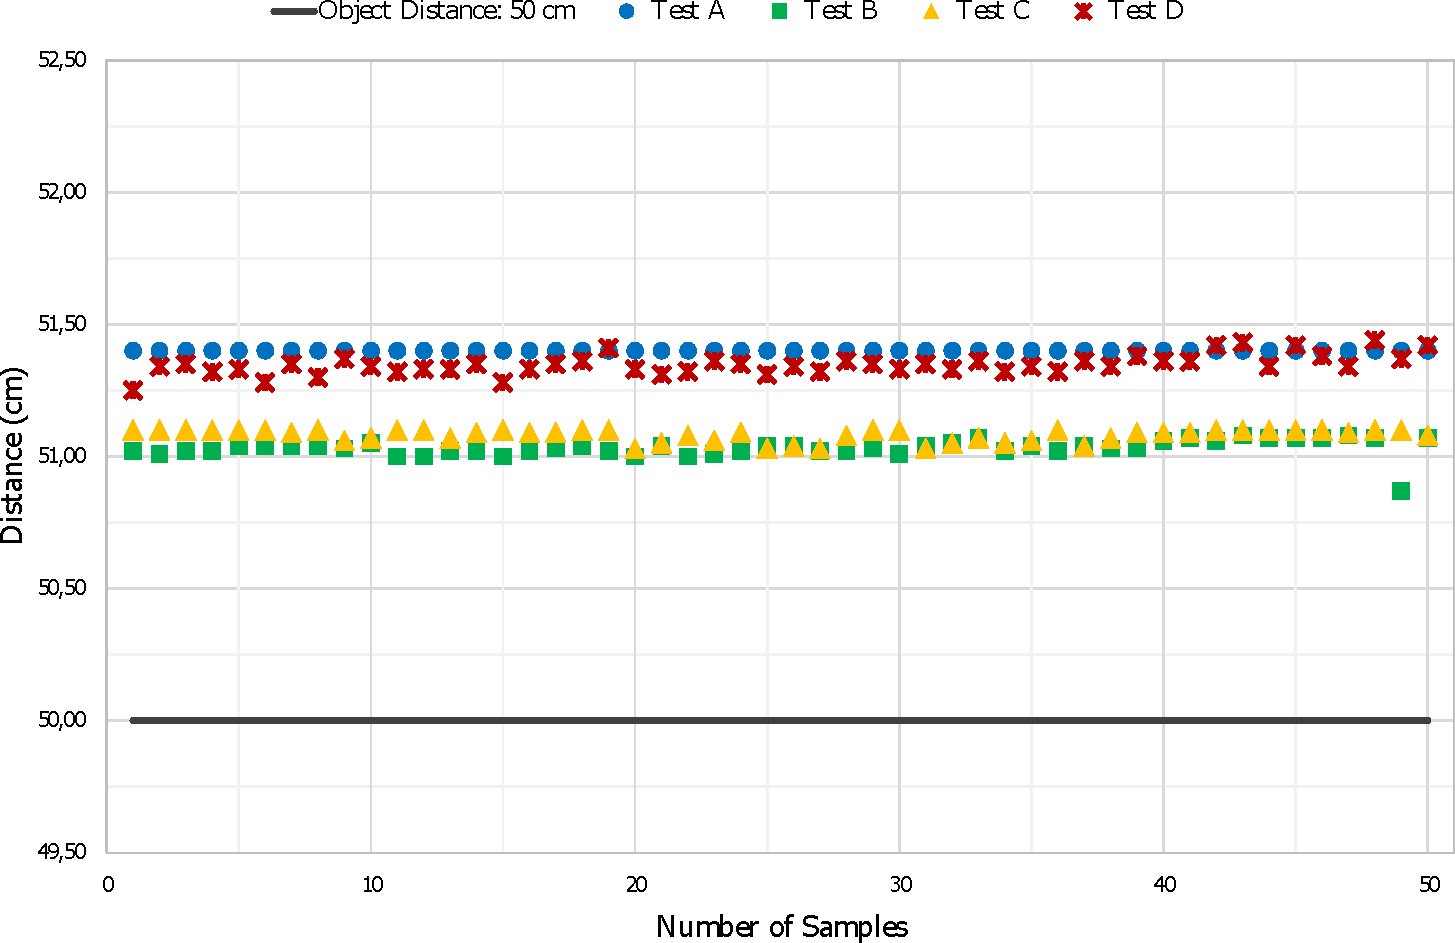
\includegraphics[scale=0.5]{images/Results/testing_methodology/50cm.pdf}
    \caption{Analysis \#1 with the object placed 50 cm from the sensor.}
    \label{fig:50cmText}
\end{figure}

Another important factor is the standard deviation, in which it could be noticed that, even for distances shorter than 100 cm, all tests provided low rates of the variation, indicating that the values tend to be close to the mean of the set. 

\begin{figure}[h!]
    \centering
    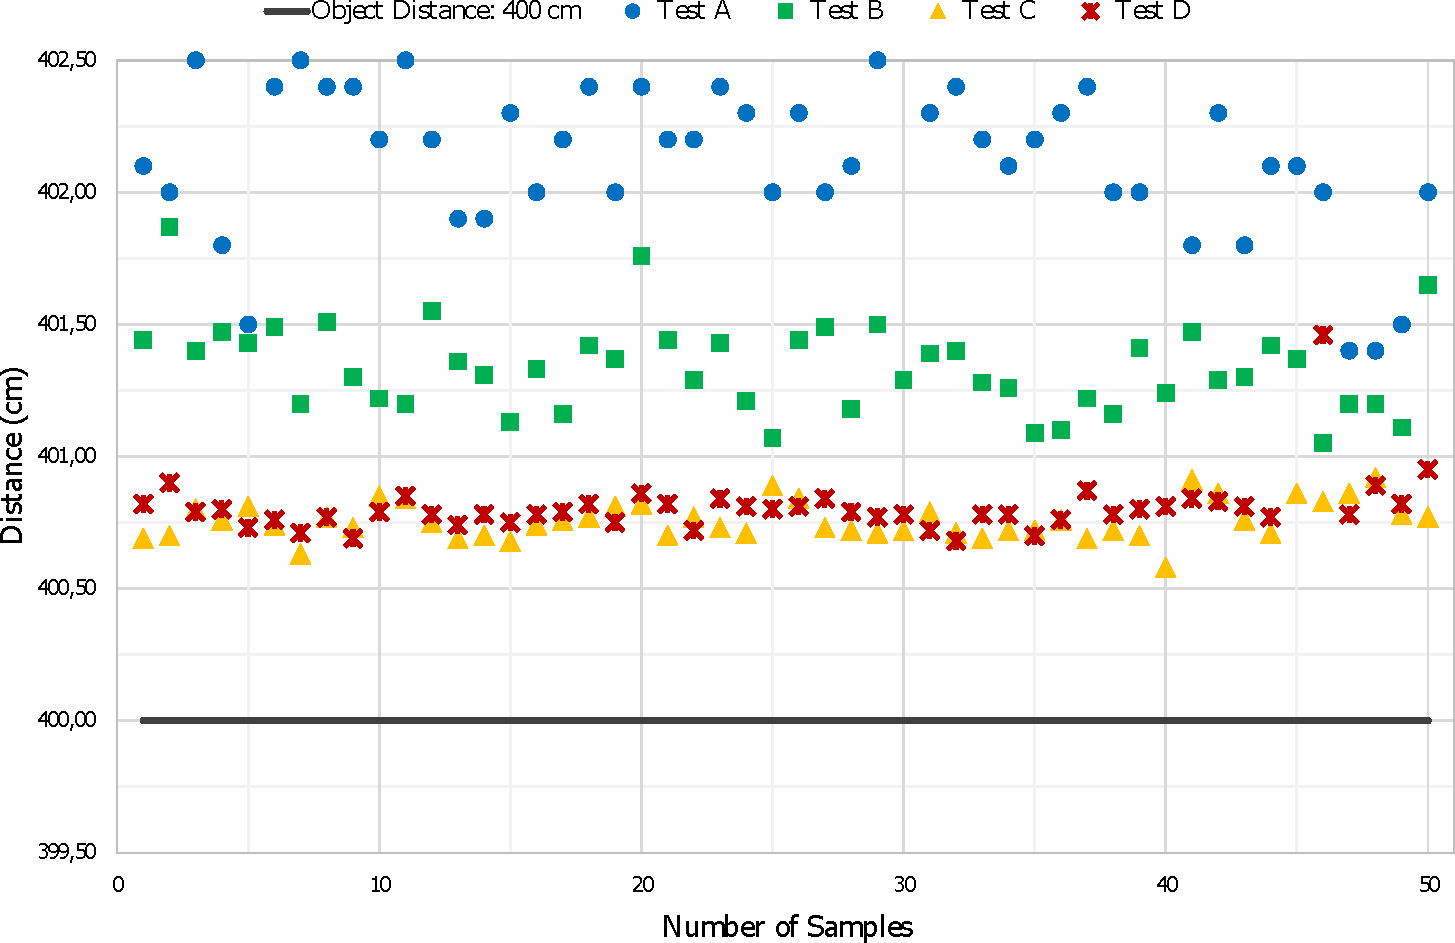
\includegraphics[scale=0.5]{images/Results/testing_methodology/400cm.pdf}
    \caption{Analysis \#1 with the object placed 400 cm from the sensor.}
    \label{fig:400cmText}
\end{figure}

Already for greater distances, the tests provided better results for the tests C and D, as the values from the tests A and B are spread out over the range, which proves that, successively measurements taken from the ultrasonic sensors decrease with higher numbers of collected samples. Figure~\ref{fig:400cmText} shows the test results, with the object placed in a distance of 400 cm. It can be noticed that, for the tests A and B, the values of each sample are scattered along the graph, differently than the results from the test C and D.

The Figure~\ref{fig:systematicError} presents the systematic error from all tests performed. It can be noticed that test A has demonstrated highest values, in which decrease successively until test D.

\begin{figure}[h!]
    \centering
    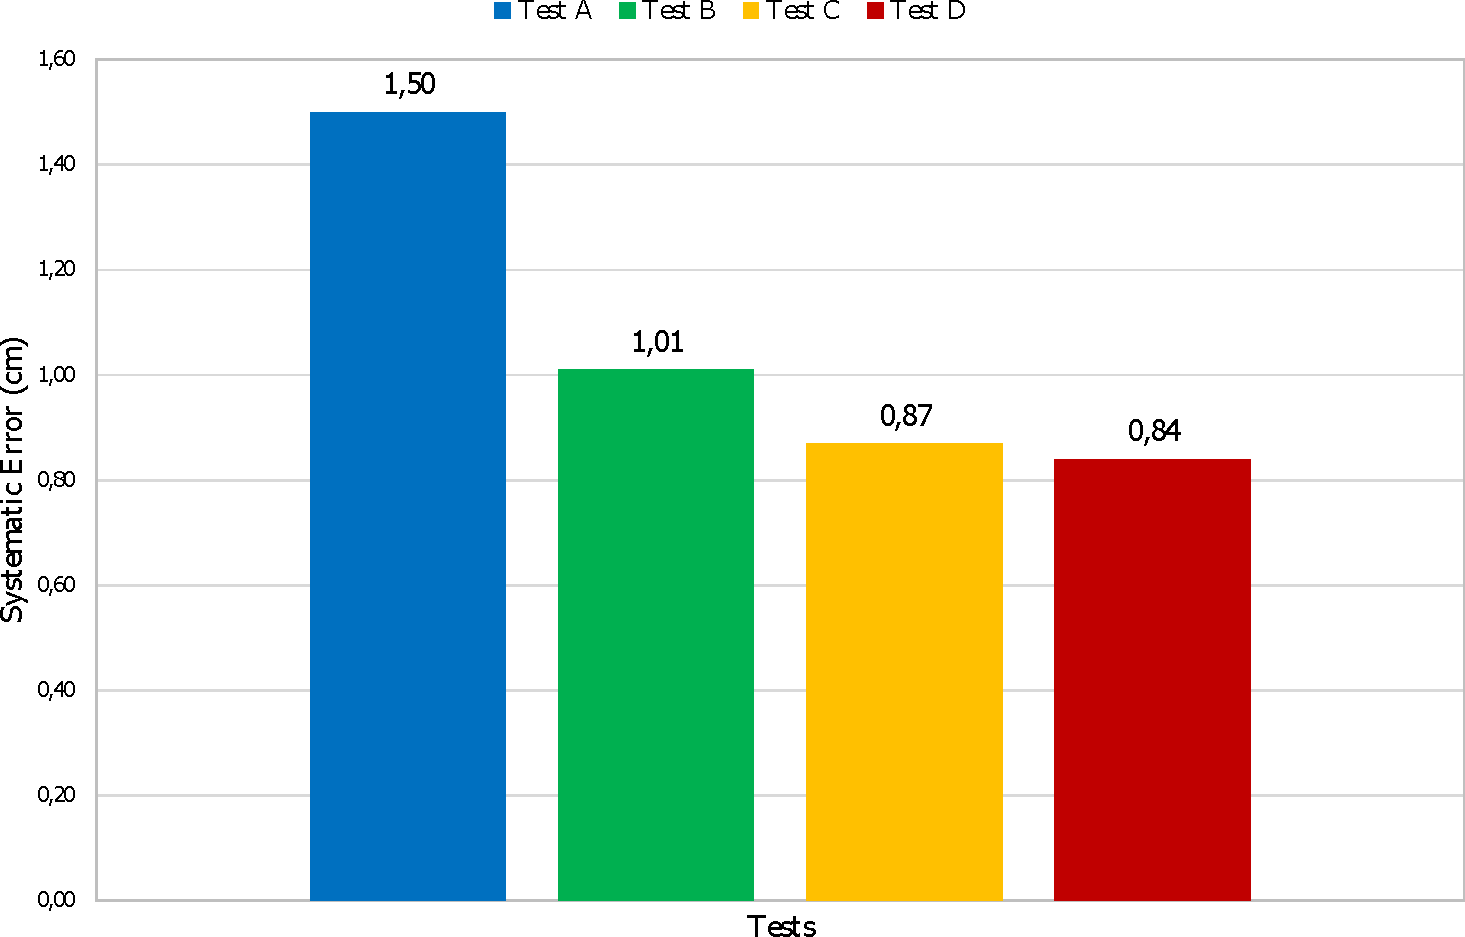
\includegraphics[scale=0.43]{images/Results/testing_methodology/systematicError.pdf}
    \caption{Average systematic error presented from all the experimental results (see Appendix \ref{appendice1:first}).}
    \label{fig:systematicError}
\end{figure}

Therefore, from the analysis, the test C and D has demonstrated promising results, principally for the test D, in which it has shown the lowest systematic error and standard deviation. However, everything comes with a cost and, in this case, the cost is the time that the ultrasonic sensor takes the readings. If the liquid's level surface changes while the sensor is reading, it may directly influence on the results of the measures. 

Using a digital oscilloscope, it was possible to evaluate this time value. For the test A, the time is 50 ms for each reading. Already for test B, it is around 250 ms. The test C, the value of the readings is 1.1 s and, for test D, the time is around 2.6 s. Therefore, using higher values of samples, as the ones used for the test D, may have a direct impact on the readings. As the detergent's liquid level does not change quickly, it would be affordable for this application to use the values approached by test D. However, if the readings are showing variations, it would be interesting to reduce the number of samples, in order to make the readings from the ultrasonic sensor faster.

After this set of tests, the best number of samples to be used as default, in terms of systematic error and standard deviation, is the one that is used on test D. Even for distances up to 400 cm, the system has demonstrated some good results, evidencing that the device may be used for reservoirs with higher heights.


\section{System's Reliability}\label{section:systemReliability}

This section will approach the reliability of the system, e.i., if the system is able to take the measurements, for a long period of time, without detecting fail readings. For this purpose, the device was submitted to take 1000 measures, within a range of distances from 10 cm to 90 cm. Higher values will not be considered, due to fact that the reservoirs from the \gls{SCMB} have height of 92 cm. Thus, it is performed some statistical analysis, in order to provide the system's accuracy.

In order to simplify the analysis process, it is chosen only three cases wherein the the object is placed 10 cm, 50 cm and 90 cm from the sensor, represented by Figures \ref{fig:conf10TEXT}, \ref{fig:conf50TEXT} and \ref{fig:conf90TEXT}, respectively. The rest of the results can be found in Appendix \ref{appendice1:second}. 

\begin{figure}[h!]
    \centering
    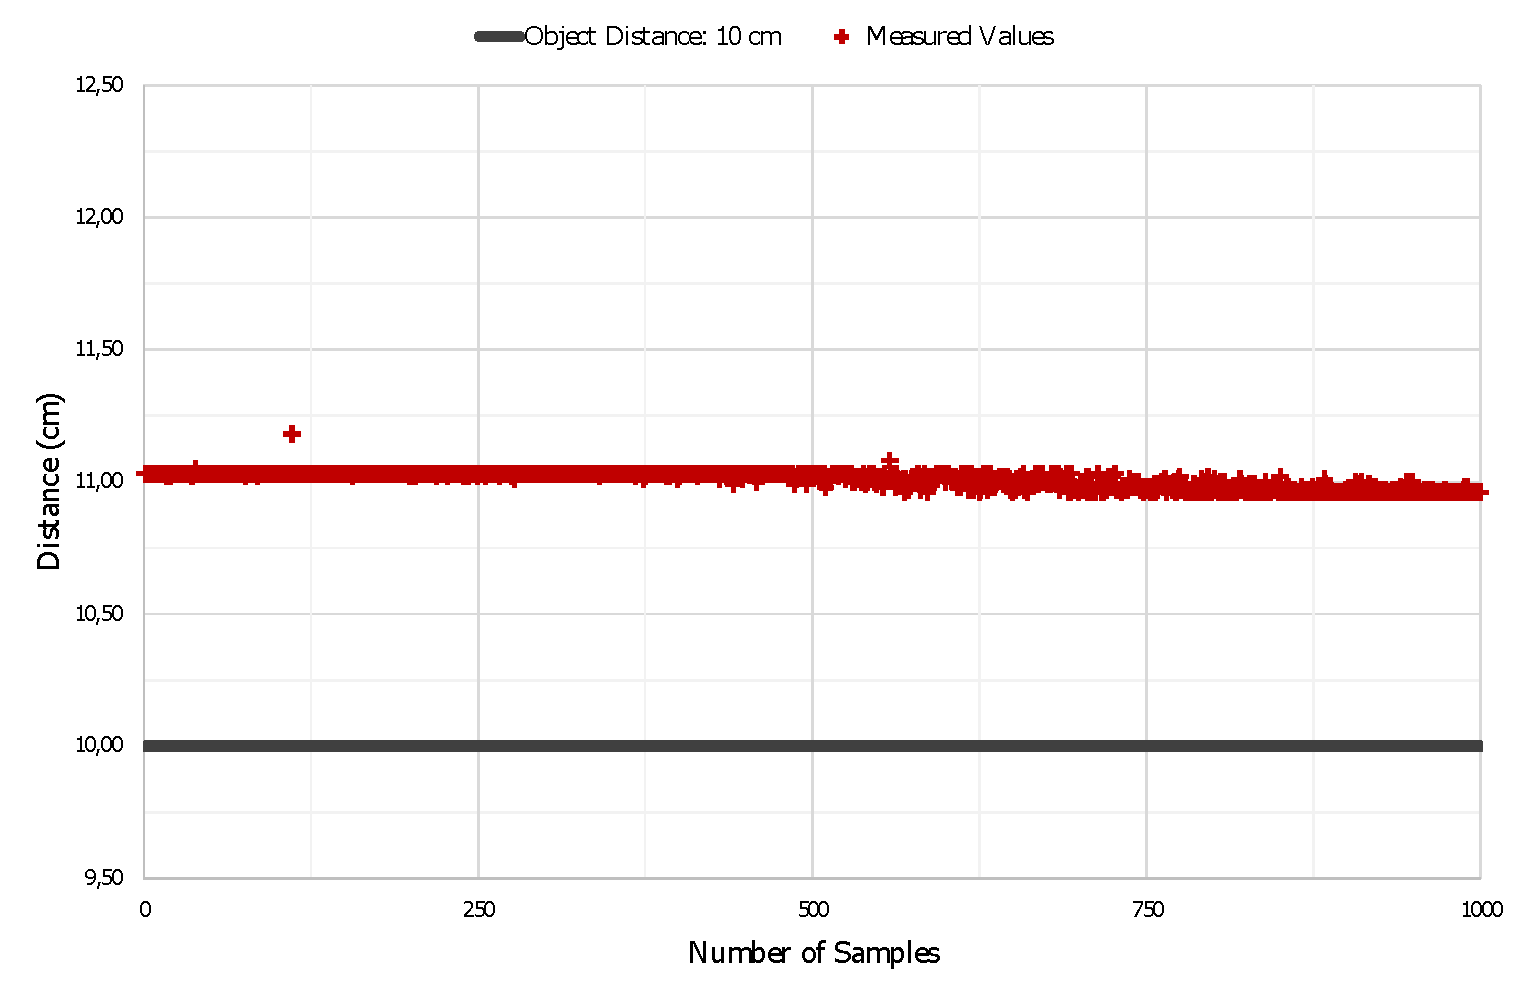
\includegraphics[scale=0.5]{images/Results/testing_methodology/conf10.pdf}
    \caption{Analysis \#2 with the object placed 10 cm from the sensor.}
    \label{fig:conf10TEXT}
\end{figure}

\begin{figure}[h!]
    \centering
    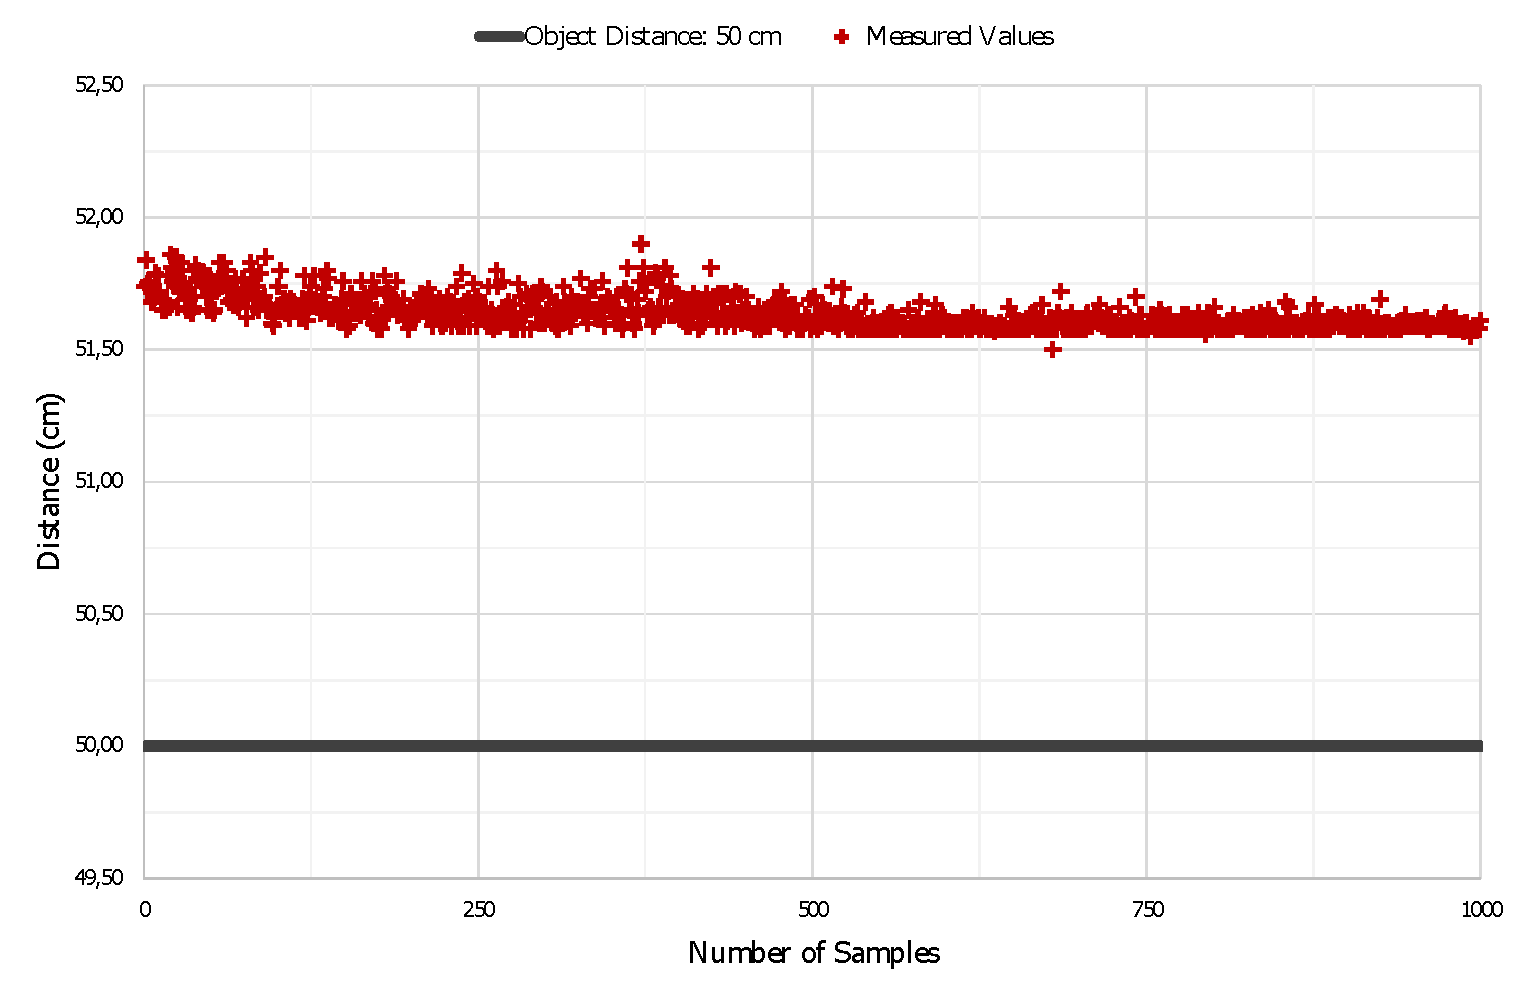
\includegraphics[scale=0.5]{images/Results/testing_methodology/conf50.pdf}
    \caption{Analysis \#2 with the object placed 50 cm from the sensor.}
    \label{fig:conf50TEXT}
\end{figure}
\clearpage
\begin{figure}[h!]
    \centering
    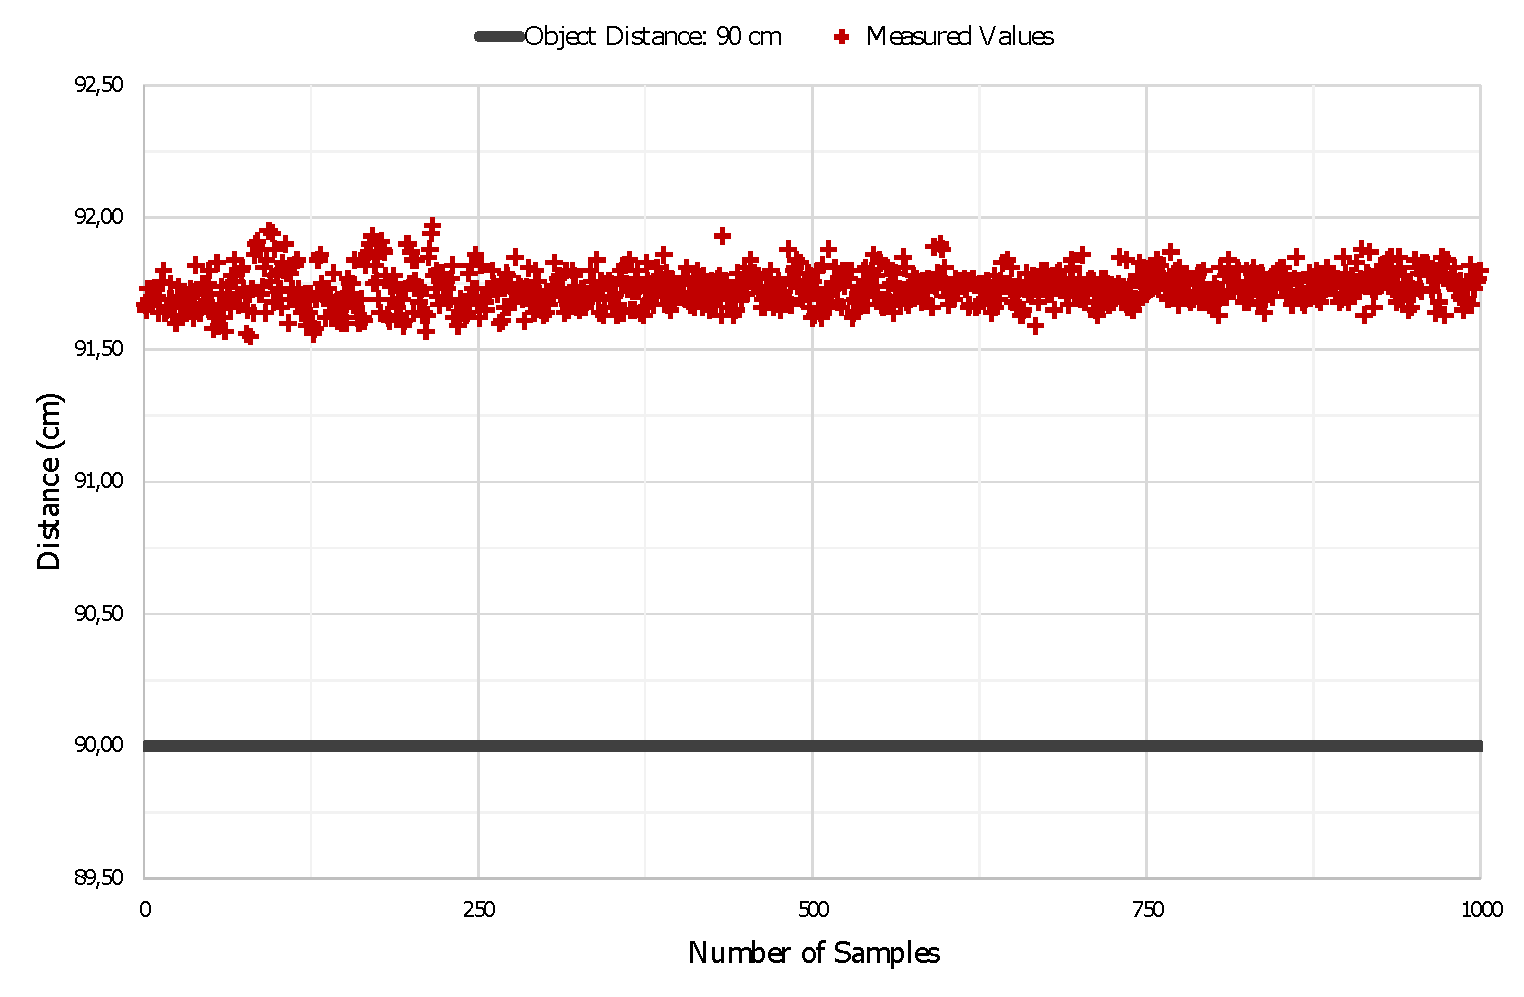
\includegraphics[scale=0.5]{images/Results/testing_methodology/conf90.pdf}
    \caption{Analysis \#2 with the object placed 90 cm from the sensor.}
    \label{fig:conf90TEXT}
\end{figure}

The Table~\ref{table:samples1000} presents the object distance, the mean values of the samples $\bar{x}$, the standard deviation $\sigma_s$, the systematic error $S_E$ and the relative error $\varepsilon$ of the 1000 samples taken. 

\begin{table}[h!]
    \centering
    \begin{tabular}{@{}ccccc@{}}
        \toprule
        \textbf{Distance (cm)} & \textbf{$\bar{x}$} (cm)& \textbf{$\sigma_s$} (cm) & \textbf{$S_E$} (cm) & \textbf{$\varepsilon$} (\%)\\ \midrule
        \rowcolor[HTML]{EFEFEF} 
        90 & 91.73 & 0.07 & 1.73 & 1.92 \\
        50 & 51.63 & 0.06 & 1.63 & 3.27 \\
        \rowcolor[HTML]{EFEFEF} 
        10 & 11.01 & 0.03 & 1.01 & 10.08 \\ \bottomrule
    \end{tabular}
    \caption{Summary of the result values presented from the 1000 samples collected.}
    \label{table:samples1000}
\end{table}

As can be noticed, for longer distances, the samples has demonstrated higher values of standard deviation $\sigma_s$, principally when comparing with shorter distances. This is an expected result, due to the fact the ultrasonic waves are travelling for longer distances. Taking a close look at the relative error $\varepsilon$, shorter distances have presented higher values, as the variations for small distances will have a significant impact, on the relative error, than for longer distances. 

In order to make a better assessment of the measurements, it will be selected 15 random values from the 1000 samples collected, and the system measurement will be evaluated with a confidence interval of 95~\%. As approached by \cite{NETO:2012}, measurement results $MR$ can be evaluated through the Equation~\ref{eq:measurementResult}

\begin{equation}\label{eq:measurementResult}
    MR = \bar{x} - S_E~\pm~\frac{Re}{\sqrt{n}}
\end{equation}
where $n$ is the number of samples and $Re$ is the repeatability of a measurement instrument, defined by the Equation~\ref{eq:repetitively}

\begin{equation}\label{eq:repetitively}
    Re = \pm~t~_x~\sigma_s
\end{equation}
in which t is the Student t-distribution.

Therefore, for a $n = 15$ samples, considering one degree of freedom ($n$ - 1) = 14 and 95\% of probability, from the table of t-distribution \cite{NETO:2012}, it is found that $t = 2.14$. Thereby, it is possible to find the repeatability of the system and define the measurement system results. Its results is demonstrated in Table~\ref{table:mr}.

\begin{table}[h!]
    \centering
    \begin{tabular}{@{}cccccc@{}}
        \toprule
        \textbf{Distance (cm)} & \textbf{$\bar{x}$ (cm)} & \textbf{$\sigma_s$ (cm)} & \textbf{$S_E$ (cm)} & \textbf{$Re$ (cm)} & \textbf{MR (cm)} \\ \midrule
        \rowcolor[HTML]{EFEFEF} 
        90 & 91.71 & 0.06 & 1.71 & 0.1 & 90.00 $\pm$ 0.03 \\
        50 & 51.65 & 0.07 & 1.65 & 0.1 & 50.00 $\pm$ 0.03 \\
        \rowcolor[HTML]{EFEFEF} 
        10 & 11.02 & 0.02 & 1.02 & 0.04 & 10.00 $\pm$ 0.01 \\ \bottomrule
    \end{tabular}
    \caption{Measurement system result using a confidence interval of 95 \% and a t-distribution of $t$ = 2.14 \cite{NETO:2012}.}
    \label{table:mr}
\end{table}

From the analysis, it can be noticed that, for the distances 90 and 50 cm, there are 95~\% of probability that the resultant values from the measurements would be within the range of $\pm$ 0.03 cm. Already for the distance of 10 cm, the range is shorter, presented a range of values within $\pm$ 0.01 cm. These values represent positive results, indicating that the accuracy of the measurement system, from the developed device, is in agreement for the detergent supervision application.


\section{Analysis of the Temperature Influence}\label{section:temperatureInfluence}

As it is more interesting, for the client, to know about the capacity and volume of the reservoir than the distance measured from the sensor, in this section, it will be approached the influence of the temperature on the reservoir capacity measured by the sensor, once it is not being used a temperature sensor. Also, it is important to highlight that reservoirs are kept in a close environment, so the temperature variation presented here are only for comparison effects.

Using the \textit{MATLAB} software, it was possible to evaluate the capacity variation as a function of the temperature. As can be seen in Figure~\ref{fig:test_temperature}, it is analyzed three tests with the capacity of the reservoir being at 5~\%, which is considered one of the cases where the temperature will have significant influence on the capacity measured. Thereby, for the test A, the temperature set in the ESP32 Module is 15ºC, for test B, 20ºC and for test C, 25ºC. Thus, the temperature is varied in a range of 5ºC to 35ºC.

\begin{figure}[h!]
    \centering
    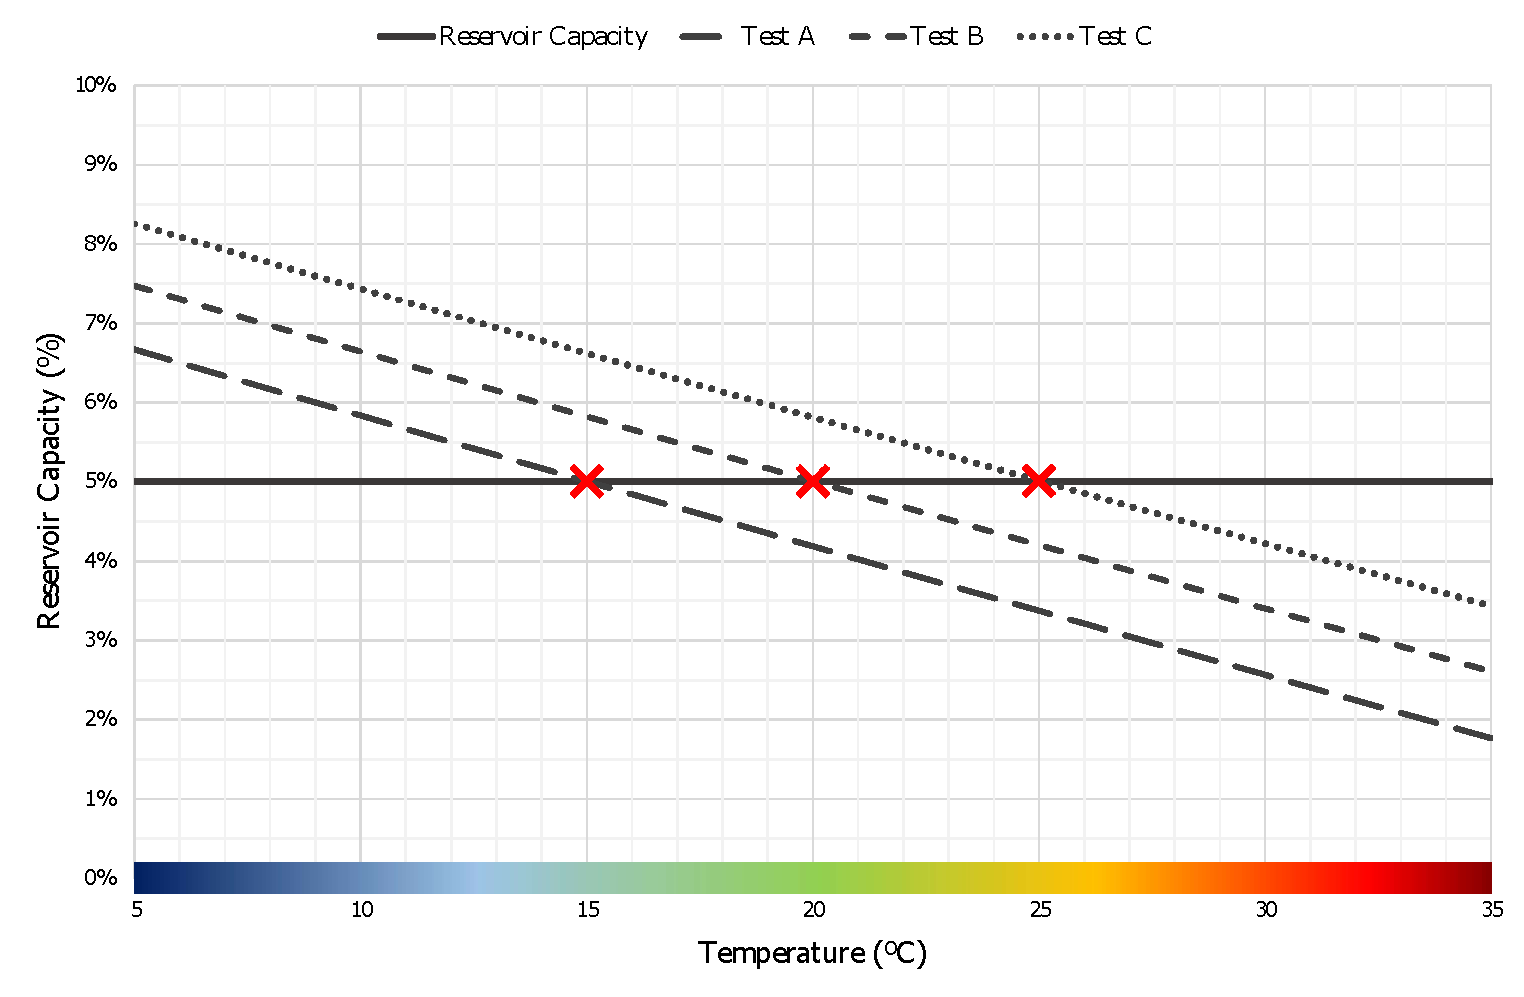
\includegraphics[scale=0.55]{images/Results/temperature_influence/Analyse_5.pdf}
    \caption{Reservoir Capacity: 5 \%; Test A: 15ºC; Test B: 20ºC; Test C: 25ºC.}
    \label{fig:test_temperature}
\end{figure}

From the analysis, the best case happens when the environment temperature is the same as the one programmed at the ESP32 Module, where the device detects the exact level measurement of the reservoir. In mostly normal conditions, the variation on the capacity would be around $\pm$ 1~\%. However, when extrapolating the variation of the temperature for 35ºC, the system would detect an maximum error slightly above 3~\%. 

In Appendix \ref{appendice1:third}, it can be found others cases where it was analyzed the capacity variation with the reservoir being at 50~\% and 95~\%. The results of the variation presented was around 1~\%, for the reservoir capacity being at 50~\%, and practically null for the reservoir that is almost full.

Therefore, the temperature sensor is not so important in this kind of application, as it will have a minimum impact on the capacity measurements. Although, in applications where the variation of 1 \%, in the reservoir's capacity, is important, it would be interesting to evaluate the use of a temperature sensor.


\section{Battery Performance}\label{section:batteryPerformance}

In order to have an assessment of the battery performance, first, it is important to point out that, the time for the system to update the \textit{status} of the detergent level on the database, may differ according to the stringency criteria that the application requires. 

The time value that the sensor will take the readings, is best estimate by implementing the system on the reservoirs at the \gls{SCMB}, and evaluate the time that would provide the best conditions, both for the battery usage and, for the readings.

Therefore, it is more interesting to talk about how many measurements (readings) the system is able to make. After some practical tests, it was possible to evaluate that, the system can make readings and update the information on the database around 9300 times. If the stringency criteria of the information to be updated is high, it would be interesting to use another battery connected, in parallel, in order to make the working time of the device longer or, it is possible to use it plugged directly with a 5 V charger, with a maximum current output of 1 A.

\section{Overall Considerations}\label{section:overallConsiderations}

In this section, it will be presented some basic considerations about the solution adopted for the detergent supervision.

First, as any \gls{IoT} application, the device must be 100~\% of the time connected with a network, otherwise, the system will no longer be able to take the readings and update the information on the database. In case the internet access is not available, some adjusts can be made, with the objective of making the ESP32 Module to save the values from the readings on its internal memory and, when the internet access becomes available again, the system would update the information all at once. Although it would be an interesting solution, for the time period that the system is offline, it would not be considered a real-time monitoring solution.

The Web platform developed in this work does not make use of any \gls{API} protection. This means that the \gls{API}s may be target of security threats and, additional vulnerabilities, due to the none use of authentication and lack of encryption. Therefore, the use of Simple Object Access Protocol (SOAP) or Representational State Transfer (REST) would be interesting in order to deal with transactional massaging security considerations, principally using an authentication and authorization architecture.

Another point to be considered is regard to the environment where the device will be placed. In the laundries facilities of the \gls{SCMB}, it is used five types of products to clear the clothes, e.g., liquid detergent, chlorinated and oxygenated blancher, neutral detergent and softener. Therefore, the device must be evaluated in order to check if the environment is being aggressive for the equipment and, if the measurements is going to be affected in the course of time. 

\section{System Cost and Architecture Proposal}\label{section:systemCost}

This section will provide an overview of the price of the components used for the work development. The values of the plastic usage (PLA) for the printing process and the wiring connections will not be considered. Moreover, the services provided from the \textit{000webhost}, for the database storage, is free, although with a limit of disk usage up to 1 GB.

From the Table~\ref{table:cost}, it can be noticed that the developed integrated system provides a low-cost \gls{IoT} solution for industrial washing machines, with prices varying around 8 to 9 \euro. Due to the number of functionalities and the reliability performed from the tests analysis, it makes the product a very interesting solution for the measurement level.

\begin{table}[h!]
    \centering
    \begin{tabular}{@{}ccc@{}}
        \toprule
        \textbf{Items} & \textbf{Quantity} & \textbf{Price (\euro)} \\ \midrule
        \rowcolor[HTML]{EFEFEF} 
        ESP32 Development Kit v1 & 1 & 3.54 \\
        US-015 Ultrasonic Sensor & 1 & 0.52 \\
        \rowcolor[HTML]{EFEFEF} 
        DC-DC Boost Converter 3 V to 5 V & 1 & 0.61 \\
        03962A Li-Ion Battery Charger & 1 & 0.16 \\
        \rowcolor[HTML]{EFEFEF} 
        LIR18650 2600 mAh & 1 & 3.50 \\
        Battery Case Holder & 1 & 0.52 \\ \hline
        \rowcolor[HTML]{EFEFEF} 
        \textbf{Total} & - & \textbf{8.85} \\ \bottomrule
    \end{tabular}
    \caption{Price table of the electronic components used. \textit{Prices based on Aliexpress and eBay (October, 2019)}.}
    \label{table:cost}
\end{table}

The advantages of having a low-cost device is the scalability, as its application can be transferred for others reservoirs, making the production more flexible. Also, it will improve the efficiency of the productive process, as it can be add actuators that can pump the liquid from spare reservoirs when a low level of capacity is detected. This \gls{IoT} Ecosystem is illustrated in Figure~\ref{fig:final}, where all the reservoirs are connected with the device developed, and all the information may be accessed through different platforms.

\begin{figure}[h!]
    \centering
    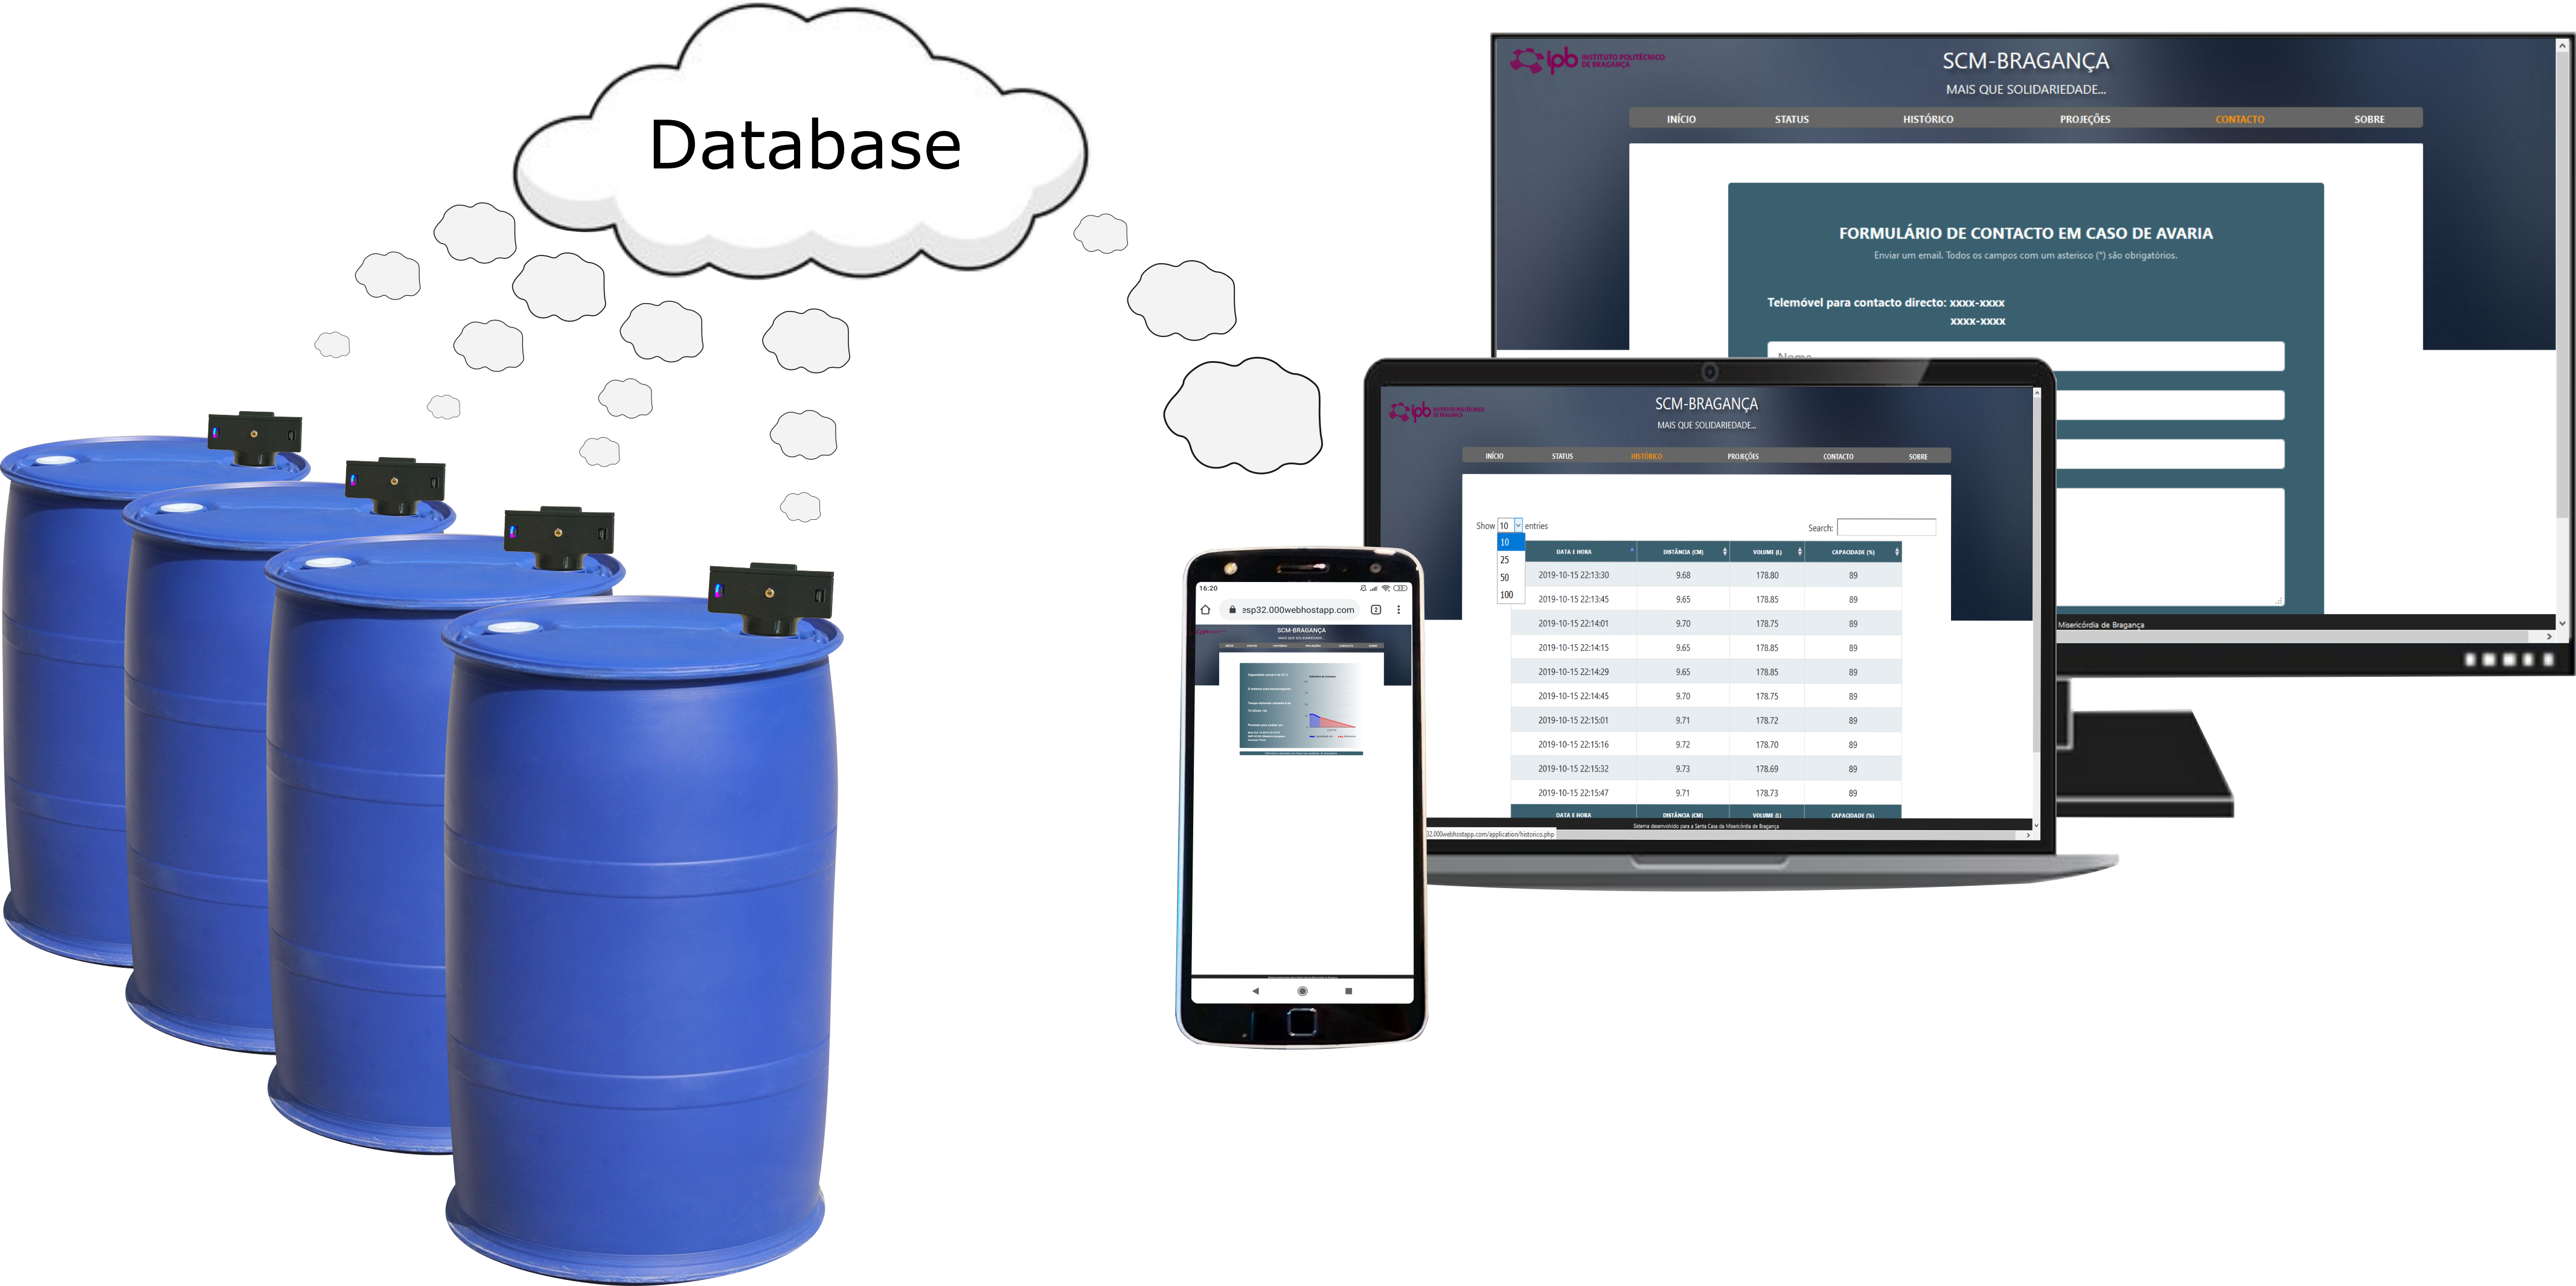
\includegraphics[scale=0.13]{images/Results/modeloFinal.png}
    \caption{IoT Ecosystem for Industrial Washing Machines.}
    \label{fig:final}
\end{figure}